% **************************************************
% Document Class Definition
% **************************************************
\documentclass[%
    paper=A4,               % paper size --> A4 is default in Germany
    twoside=true,           % onesite or twoside printing
    openright,              % doublepage cleaning ends up right side
    parskip=full,           % spacing value / method for paragraphs
    chapterprefix=true,     % prefix for chapter marks
    11pt,                   % font size
    headings=normal,        % size of headings
    bibliography=totoc,     % include bib in toc
    listof=totoc,           % include listof entries in toc
    titlepage=on,           % own page for each title page
    captions=tableabove,    % display table captions above the float env
    draft=false,            % value for draft version
]{scrreprt}%

% !TEX root = main.tex
% chktex-file 46

% **************************************************
% Files' Character Encoding
% **************************************************
\PassOptionsToPackage{utf8}{inputenc}
\usepackage{inputenc}
\usepackage[english,ngerman]{babel}

% **************************************************
% Information and Commands for Reuse
% **************************************************
\newcommand{\thesisTitle}{Probabilistische online Wissensgraphkonstruktion aus natürlicher Sprache}
\newcommand{\thesisName}{Clemens Damke}
\newcommand{\thesisMatNr}{7011488}
\newcommand{\thesisSubject}{Bachelorarbeit}
\newcommand{\thesisDate}{\today}
\newcommand{\thesisVersion}{Entwurf 1}

\newcommand{\thesisFirstReviewer}{Prof.~Dr.~Eyke Hüllermeier}
\newcommand{\thesisFirstReviewerUniversity}{\protect{Universität Paderborn}}
\newcommand{\thesisFirstReviewerDepartment}{Institut für Informatik}

\newcommand{\thesisSecondReviewer}{Prof.~Dr.~Axel-Cyrille Ngonga Ngomo}
\newcommand{\thesisSecondReviewerUniversity}{\protect{Universität Paderborn}}
\newcommand{\thesisSecondReviewerDepartment}{Institut für Informatik}

\newcommand{\thesisFirstSupervisor}{Dr.~Theodor Lettmann}
\newcommand{\thesisSecondSupervisor}{Prof.~Dr.~Eyke Hüllermeier}

\newcommand{\thesisUniversity}{Universität Paderborn}
\newcommand{\thesisUniversityDepartment}{}
\newcommand{\thesisUniversityInstitute}{Institut für Informatik}
\newcommand{\thesisUniversityGroup}{Intelligente Systeme}
\newcommand{\thesisUniversityCity}{Paderborn}
\newcommand{\thesisUniversityStreetAddress}{Pohlweg 51}
\newcommand{\thesisUniversityPostalCode}{33098}


% **************************************************
% Debug LaTeX Information
% **************************************************
%\listfiles


% **************************************************
% Load and Configure Packages
% **************************************************

% Colors:
\usepackage[usenames, dvipsnames, svgnames, table]{xcolor}

\definecolor{blau}{HTML}{355FB3}
\definecolor{rot}{HTML}{B33535}
\definecolor{gruen}{HTML}{3BB335}
\definecolor{dunkelblau}{HTML}{1E3666}
\definecolor{hellblau}{HTML}{8ea7d7}

\PassOptionsToPackage{% setup clean thesis style
    figuresep=space,
    sansserif=false,
    hangfigurecaption=false,
    hangsection=true,
    hangsubsection=true,
    colorize=full,
    colortheme=custom,
	colormain=dunkelblau,
	coloraccessory=blau,
    bibsys=bibtex,
    bibfile=bib-refs,
    bibstyle=alphabetic,
    wrapfooter=false,
}{cleanthesis}
\usepackage{cleanthesis}

\usepackage{mathtools}
\newcommand\numberthis{\addtocounter{equation}{1}\tag{\theequation}}

\usepackage{graphicx}
\usepackage{tikz}
\usetikzlibrary{arrows,positioning}
\usetikzlibrary{calc}
\newcommand{\tikzmark}[1]{\tikz[overlay,remember picture] \node (#1) {};} % chktex 1

\usepackage{pgfplots}
\usepackage{pgfplotstable}
\pgfplotsset{compat=1.14}
\usepgfplotslibrary{dateplot, statistics}
\pgfplotsset{
    cycle list={blau\\rot\\gruen\\},
}

\usepackage{listings}
\lstset{basicstyle=\ttfamily,breaklines=true}

\usepackage[bguq]{frege}
\usepackage{stmaryrd}
\usepackage{multicol}
\usepackage{pbox}
\usepackage{xifthen}

\hypersetup{% setup the hyperref-package options
    pdftitle={\thesisTitle},    %   - title (PDF meta)
    pdfsubject={\thesisSubject},%   - subject (PDF meta)
    pdfauthor={\thesisName},    %   - author (PDF meta)
    plainpages=false,           %   -
    colorlinks=false,           %   - colorize links?
    pdfborder={0 0 0},          %   -
    breaklinks=true,            %   - allow line break inside links
    bookmarksnumbered=true,     %
    bookmarksopen=true          %
}

\makeatletter
\newcounter{rulecount}[section]
\newcommand{\rulemark}[1]{\ensuremath{\refstepcounter{rulecount}(r_{\therulecount})\ltx@label{#1}}} % chktex 36
\newcommand{\ruleref}[1]{\ensuremath{r_{\ref{#1}}}}
\makeatother


% **************************************************
% Document CONTENT
% **************************************************
\begin{document}

% --------------------------
% rename document parts
% --------------------------
\renewcaptionname{ngerman}{\figurename}{Abb.}
\renewcaptionname{ngerman}{\tablename}{Tab.}

\newcommand{\fixedinput}{\input}

% --------------------------
% Front matter
% --------------------------
\pagenumbering{roman}			% roman page numbing (invisible for empty page style)
\pagestyle{empty}				% no header or footers
\input{content/titlepages}		% INCLUDE: all titlepages
\cleardoublepage\

\pagestyle{plain}				% display just page numbers
% !TEX root = ../main.tex
%
\pdfbookmark[0]{Abstract}{Abstract}
\chapter*{Abstract}%
\label{sec:abstract}
\vspace*{-10mm}

In dieser Arbeit wird ein Verfahren zur automatisierten Wissensgraph-Konstruktion aus natürlichsprachlichen textuellen Kommunikationsdaten (z.~B. E-Mails) vorgestellt.
Das vorgestellte Verfahren transformiert einen Stream von Textnachrichten sukzessive in einen Wissensgraphen.
Es arbeitet in zwei Schritten:
Im ersten Schritt wird ein Natural Language Processing (NLP) einer eingegebenen Nachricht mit der Stanford CoreNLP Bibliothek durchgeführt.
Das im NLP-Schritt extrahierte Wissen wird anschließend mittels der Probabilistic Soft Logic (PSL) in den vorhandenen Wissensgraphen eingefügt, der aus vorhergehenden Nachrichten konstruiert wurde.
Die Struktur des so konstruierten Graphen baut auf J.~F.~Sowas Konzeptgraphen auf.
Neu in dieser Arbeit ist die Kombination von Konzeptgraphen, CoreNLP und PSL.\@
Der Vorteil dieser Kombination ist die hohe Ausdrucksstärke der konstruierten Wissensgraphen und die Skalierbarkeit des Verfahrens.
Das Verfahren wurde implementiert und wird anhand realer Testdaten bewertet.
		% INCLUDE: the abstracts (english and german)
\cleardoublepage\
%
\setcounter{tocdepth}{2}		% define depth of toc
\tableofcontents				% display table of contents
\cleardoublepage\
% --------------------------
% Body matter
% --------------------------
\pagestyle{maincontentstyle} 	% fancy header and footer

% !TEX root = ../main.tex
%
\chapter{Einleitung}
\label{sec:intro}

\cleanchapterquote{
The actual world cannot be distinguished from a world of imagination by any description.
Hence the need of pronoun and indices, and the more complicated the subject the greater the need of them.
}{Charles Sanders Peirce}{Mathematiker und Philosoph}

\section{Motivation}
\label{sec:intro:motivation}

In den letzten Jahren hat die Repräsentation von Wissensbasen durch Graphen, sog. Wissensgraphen, immer mehr an Bedeutung gewonnen.
Google, Bing und IBM Watson benutzen solche Wissensgraphen z.~B. zum Beantworten von komplexen Suchanfragen.

Die Grundidee dabei ist es, Entitäten durch Knoten und Relationen durch Kanten abzubilden.
Entitäten können konkrete Dinge, wie z.~B. Personen, aber auch abstrakte Konzepte, wie z.~B. historische Epochen, sein.
Relationen beschreiben beliebige Beziehungen zwischen den Entitäten, z.~B. \(person(\text{Da~Vinci}) \xrightarrow{\text{lived~in}} epoch(\text{Renaissance})\).
Die Entität, von der eine solche Relation ausgeht, wird als Subjekt und die Zielentität als Objekt der Relation bezeichnet.

Die Typen von Entitäten bzw.\ Relationen (z.~B. \(person\) bzw. \(lived~in\)) und deren Bedeutung sind dabei i.~d.~R. formal in einer sog.\ Ontologie spezifiziert.
Die Ontologie beschränkt also die Menge gültiger Wissensgraphen, was eine effiziente maschinelle Verarbeitung der im Graph enthaltenen Informationen ermöglicht.

Da Wissensgraphen in zahlreichen Domänen einsetzbar sind, wird deren automatisierte Konstruktion bereits seit Jahren erforscht.
Manuelles Konstruieren und vor allem anschließendes Warten und Aktualisieren von Wissensgraphen, ist aufgrund der abzubildenden Datenmengen nicht praktikabel.
Bei einer maschinellen automatisierten Konstruktion sind insbesondere zwei Anforderungen problematisch:
\begin{enumerate}
	\item Das Verarbeiten von unstrukturierten Eingaben, wie z.~B. natürlichsprachlichen Texten.
	\item Effizientes Eingliedern neuer Informationen in einen bestehenden Wissensgraphen.
		Dieses Eingliedern von Informationen umfasst im Speziellen:
		\begin{itemize}
			\item \textbf{Entity Resolution:}
				Hinzukommende Entitäten, die bereits im Graphen enthalten sind, müssen als Duplikate erkannt werden.
				Dies ist i.~d.~R. nicht trivial, da die selbe Entität durch viele verschiedene, oftmals vom Kontext abhängige, Token repräsentiert werden kann;
				z.~B. \textit{Bob} vs. \textit{Robert} oder \textit{Der Papst} vs. \textit{Franziskus}.
			\item \textbf{Link Prediction:}
				Hinzukommende Entitäten müssen mit bereits bestehenden Entitäten in Relation gesetzt werden.
				Hinzukommende Relationen können zudem benutzt werden um andere Relationen zu inferieren;
				z.~B. \[female(A) \land B \xrightarrow{\text{son~of}} A \implies A \xrightarrow{\text{mother~of}} B\]
		\end{itemize}
\end{enumerate}

Die Kombination dieser beiden Anforderungen ist interessant, da das meiste verfügbare Wissen in natürlichsprachlicher Textform vorliegt und zudem permanent neues Wissen entsteht.
Ein automatisiertes Wissensgraphkonstruktionsverfahren, welches beide Anforderungen berücksichtigt, ist daher in diversen Domänen von Nutzen.
Ein Beispiel hierfür ist die Auswertung von Kommunikationsdaten aus E-Mails oder Chat-Nachrichten mit dem Ziel die sozialen Beziehungen und Intentionen der Kommunikationpartner zu ermitteln.

\section{Ziele der Arbeit}
\label{sec:intro:goals}

Das übergeordnete Ziel dieser Arbeit ist es, ein Verfahren zu finden, welches das soeben beschriebene Problem der automatisierten Wissensgraphkonstruktion für E-Mail-Daten löst.
Konkret sei ein Stream von E-Mails gegeben, denen jeweils ein Inhalt, ein Absender, eine Menge von Empfängern und ggf.\ weitere Metadaten, wie z.~B. Absendezeit, Absendeort oder IP-Adresse, zugeordnet ist.
Die Nachrichteninhalte werden der Einfachheit halber als ausschließlich englischsprachig angenommen.
Außerdem wird eine, für E-Mails und andere Kurznachrichten typische, eingeschränkte Sprachkomplexität angenommen.
Die Nachrichten sollen nacheinander in das zu konstruierende System eingefügt werden, welches sukzessive einen Wissensgraphen daraus erzeugt.

Für diese Erzeugung muss eine Reihe von Teilproblemen gelöst werden:
\begin{enumerate}
	\item Spezifikation einer Wissensgraphontologie, die mächtig genug ist, um die Diversität natürlichsprachlich beschriebener Informationen abzubilden.
	\item Spezifikation der maschinellen Repräsentation des Wissensgraphen.
	\item Finden eines Verfahrens, welches die natürlichsprachlichen Inhalte der Nachrichten in eine maschinell leichter zu verarbeitende Form bringt.
	\item Finden eines Verfahrens, um eine eintreffende Nachricht in den bestehenden Wissensgraphen einzufügen.
\end{enumerate}

\section{Aufbau der Arbeit}
\label{sec:intro:structure}

\textbf{Kapitel~\ref{sec:related}} \\[0.2em]

\textbf{Kapitel~\ref{sec:theory}} \\[0.2em]

\textbf{Kapitel~\ref{sec:text2kg}} \\[0.2em]

\textbf{Kapitel~\ref{sec:evaluation}} \\[0.2em]

\textbf{Kapitel~\ref{sec:conclusion}} \\[0.2em]

% !TEX root = ../main.tex
%
\chapter{Verwandte Arbeiten}
\label{sec:related}

Die in~\ref{sec:intro:goals} beschriebenen Ziele werden bereits seit langem erforscht.
Der Begriff \textit{Wissensgraph} wurde 2012 durch Google popularisiert, die Ideen dahinter lassen sich allerdings bis ins Ende des 19. Jahrhunderts zurückverfolgen.
Dieses Kapitel zeigt auf, wie sich die Themen dieser Arbeit in die bisherige Forschung einfügen.
\ref{sec:related:kr} ordnet das Konzept des Wissensgraphen in die Entwicklungsgeschichte der Wissensrepräsentation ein.
\ref{sec:related:kbc} beschreibt die aktuell verwendeten Verfahren zur Konstruktion von Wissensgraphen.
In~\ref{sec:related:nlp} wird schließlich ein Überblick über die momentan verbreiteten NLP (\textit{natural language processing}) Werkzeuge gegeben.

\section{Ansätze zur Wissensrepräsentation}
\label{sec:related:kr}

\subsection{Logische Grundlagen}
\label{sec:related:kr:logic}

Die Entwicklung der Wissensrepräsentation hängt eng mit der Entwicklung der Logik zusammen.
Während in der formalen Logik und Mathematik die Prädikatenlogik das allgemein verwendete Kalkül ist und alternative Formalismen kaum verbreitet sind, finden im Bereich der Wissensrepräsentation bis heute diverse andere Kalküle Verwendung.
Diese werden im Folgenden kurz vorgestellt.

\paragraph{Begriffsschrift (1879)}
Gottlob Freges Buch über die \textit{Begriffsschrift} gilt als eines der bedeutsamsten Werke der Logik.
Sie ist der erste Formalismus mit der Mächtigkeit der modernen Prädikatenlogik zweiter Ordnung mit Identität.
Frege benutzt hierfür eine zweidimensionale Notation, die sich stark von der heute gebräuchlichen, linearen, an die Algebra angelehnte Notation unterscheidet.
\begin{equation*}
	\vcenter{\hbox{\Fconditional[\Fanqn{a}]{\Fcontent \mathfrak{R(a)}}{\Fncontent \mathfrak{P(a)}}}}
	\quad\Leftrightarrow\quad
	\exists\ a: P(a) \lor R(a)
\end{equation*}
Im Gegensatz zur Prädikatenlogik gibt es keine eigene Syntax für \textit{UND} und \textit{ODER};
diese Operatoren müssen durch die Kombination von Negation und Implikation abgebildet werden.
Zudem gibt es ausschließlich den Allquantor;
eine existenzquantisierte Aussage muss durch Negation der negierten allquantisierten Aussage ausgedrückt werden.

\paragraph{Prädikatenlogik: Peirce Notation (1885)}
Unabhängig von Frege entwickelte der amerikanische Mathematiker Charles Sanders Peirce ebenfalls ein prädikatenlogisches Kalkül.
Peirces Notation hatte starke Ähnlichkeiten mit der heute benutzten linearen Schreibweise.
Statt den modernen Symbolen hat Peirce allerdings die algebraischen Operatoren benutzt, um die Analogien zwischen Logik und Algebra auszudrücken.
\begin{equation*}
	\Sigma_a\ P_a + R_a
	\quad\Leftrightarrow\quad
	\exists\ a: P(a) \lor R(a)
\end{equation*}

\paragraph{Existential Graphs (1897)}
Neben seiner zuvor entwickelten linearen prädikatenlogischen Notation, hat Peirce zudem viele Jahre an einem alternativen graphischen Kalkül gearbeitet, welches er \textit{Existential Graphs} (zu dt.~Existenzgraphen) nannte.
Ähnlich wie die Begriffsschrift werden Existenzgraphen zweidimensional dargestellt.
Von dieser Gemeinsamkeit abgesehen, funktionieren sie allerdings fundamental verschieden.
Ein logischer Ausdruck wird hier durch einen ungerichteten Graphen beschrieben.
Die konkrete räumliche Anordnung der Knoten und Kanten hat dabei keine semantische Relevanz.

Peirce hat Existenzgraphen als ein dreistufiges aufeinander aufbauendes System konzipiert.
Die erste Stufe, die sog.\ $\alpha$-Graphen, umfasst alle notwendigen syntaktischen Elemente, um ein Kalkül mit der Mächtigkeit der Aussagenlogik zu erhalten.
Die $\beta$-Graphen bilden die zweite Stufe und erweitern die Syntax der $\alpha$-Graphen, sodass die Mächtigkeit der Prädikatenlogik erster Ordnung erreicht wird.
Sowohl für $\alpha$-, als auch für $\beta$-Graphen, ist die Vollständigkeit und Korrektheit bewiesen.
Die dritte Stufe ($\gamma$-Graphen) wurde von Pierce nie vollendet;
sie deckt in etwa die Mächtigkeit der heutigen Prädikatenlogik höherer Ordnung sowie der Modallogik ab.
\begin{align*}
	\vcenter{\hbox{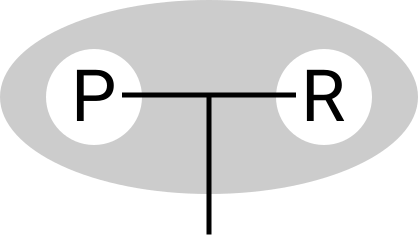
\includegraphics[height=3em]{gfx/related-work/existentialGraphExample1.pdf}}}
	\quad\Leftrightarrow\quad
	\exists\ a: P(a) \lor R(a)
\end{align*}
Wie schon die Begriffsschrift, sind Existenzgraphen syntaktisch minimal.
Direkt ausdrücken lässt sich lediglich \textit{UND}, der Existenzquantor und die Negation.
Ein weiterer Unterschied zur heutigen Prädikatenlogik ist die Beschreibung logischer Inferenzen.
Im Gegensatz zu den prädikatenlogischen Ersetzungsaxiomen, die auf der syntaktischen Struktur von logischen Ausdrücken operieren (z.~B. für Kommutativität), lassen sich die Ersetzungsaxiome für Existenzgraphen als Graphtransformationsregeln verstehen, die bestimmte Teilmengen der Knoten und Kanten eines Ausdrucks durch andere äquivalente Knoten- und Kantenmengen ersetzen.

\paragraph{Prädikatenlogik: Peano-Russell Notation (1910)}
Die zweidimensionalen Notationen wurde häufig kritisiert, da sie die lineare, algebraische Notation der symbolischen Logik von Boole und De Morgan verwarfen.
Freges Begriffsschrft und Peirces Existenzgraphen konnten sich daher nicht durchsetzen.
Peirces algebraische prädikatenlogische Notation hingegen, stieß auf größere Akzeptanz.
Giuseppe Peano hat auf deren Basis eine ähnliche Notation entwickelt, welche allerdings nicht die algebraischen Operatoren benutzt, damit sich logische Ausdrücke besser mit mathematischen Ausdrücken kombinieren lassen.
Bertrand Russell hat Peanos Notation anschließend in leicht abgewandelter Form in den \textit{Principia Mathematica} (1910) benutzt.
Diese sog.~Peano-Russell-Notation ist im Wesentlichen identisch mit der modernen Schreibweise.

Trotz des Verschwindens der zweidimensionalen Notationen, finden sich noch heute Anlehnungen daran.
So ist z.~B. die Negation $\lnot A$ auf Freges negierten Inhaltsstrich $\Fncontent A$ und der Ableitungsoperator $\vdash$ auf Freges Urteilsstrich mit angefügtem Inhaltsstrich $\Facontent$ zurückzuführen.

\subsection{Entwicklung maschineller Wissensrepräsentation}
\label{sec:related:kr:history}

Die Idee Computer zur Lösung beliebiger Probleme zu benutzen ist nicht neu.
Da ein solches maschinelles Problemlösen immer die Verfügbarkeit von Hintergrundwissen über die Problemdomäne erfordert,
wurden Methoden zur Wissensrepräsentation immer im Zusammenhang mit Problemlösern erforscht.
So wie effiziente Datenstrukturen die Implementation effizienter Algorithmen ermöglichen, ermöglichen gute Wissensrepräsentationen die Implementation guter Problemlöser.
Was genau nun als ein guter Problemlöser verstanden wird, hat sich im Laufe der Jahre allerdings immer wieder verändert.

\paragraph{Universelle Problemlöser}
Einer der ersten maschinellen Problemlöser war der von Simon, Shaw und Newell 1955 entwickelte \textit{Logic Theorist} (LT).
LT war in der Lage logische Aussagen zu beweisen, indem er systematisch Ersetzungsaxiome auf eine gegebene Aussage angewandt hat, bis die gesuchte Lösung abgeleitet wurde.

Die Grundidee des LT haben Simon, Shaw und Newell 1959 im \textit{General Problem Solver} (GPS) erweitert.
Es wurden Heuristiken hinzugefügt, um den Suchraum geschickter zu durchlaufen.
GPS war ein universeller Problemlöser, konnte also jedes Problem lösen, das sich durch eine Menge von Horn-Klauseln ausdrücken lässt.
Zwar war es so theoretisch möglich Probleme aus diversen Domänen zu lösen, aufgrund der kombinatorischen Explosion war GPS alledings nicht zur Lösung komplexer praktischer Probleme geeignet.

\paragraph{Expertensysteme}
Aufgrund der Misserfolge universeller Problemlöser für praktische Probleme, hat die Forschung begonnen sich mehr auf die Entwicklung von Expertensystemen zu fokussieren.
Expertensysteme besitzen für gewöhnlich eine Wissensbasis in der domänenspezifisches Wissen in Form von Regeln und Fakten kodiert ist.
Eine sog.~Inferenzmaschine benutzt diese Regeln und Fakten um Probleme zu lösen.

\paragraph{Semantic Networks (1956)}
Die Idee, Graphen als Datenstruktur für Wissensbasen zu verwenden, taucht erstmal in den sog.~\textit{Semantic Networks} (zu dt.~semantische Netzwerke) auf.
Dieser Ansatz beschreibt Wissen als Menge von $(subject, predicate, object)$-Tripeln.
Es gibt darüber hinaus keine klaren Regeln, wie ein semantisches Netz strukturiert sein muss.

\paragraph{Conceptual Graphs (1976)}
Wie genau mit Graphen komplexes Wissen beschrieben werden kann, das über eine reine Taxonomie hinaus geht, blieb bei semantischen Netzen unklar.
John F. Sowas \textit{Conceptual Graphs} (zu dt.~Konzeptgraphen) lösen dieses Problem.
Statt Wissen als eine Menge von Beziehungen abzubilden, wird es als prädikatenlogischer Ausdruck verstanden.
Hierfür baut Sowa auf Peirces Existenzgraphen auf, die bis dahin weitestgehend unbeachtet waren.
\begin{align*}
	\vcenter{\hbox{
\includegraphics[height=4em]{gfx/related-work/conceptGraphExample1.pdf}}}
	\quad\Leftrightarrow\quad
	\exists\ a: P(a) \lor R(a)
\end{align*}
Dieser Ansatz erlaubt es komplexe Wissensbasen zu konstruieren, in denen nicht nur gespeichert werden kann, ob ein Konzept existiert, sondern auch, ob es nicht oder nur möglicherweise existiert.
Da Konzeptgraphen, so wie schon die Existenzgraphen, ein vollständiges und korrektes Logikkalkül sind, lassen sich zudem Inferenzregeln für sie definieren.
Der Vorteil hierfür einen Graphen statt eines prädikatenlogischen Ausdrucks zu verwenden ist, dass eine Graphstruktur einen deutlich effizienteren Zugriff auf gespeichertes Wissen ermöglicht.

\paragraph{Knowledge Graphs (1987)}
Der Begriff \textit{Knowledge Graph} (zu dt.~Wissensgraph) bezeichnete ursprünglich eine Klasse semantischer Netze, deren Relationsmenge formal spezifiziert ist.
Dies schränkt die Menge erlaubter Graphen ein und ermöglicht die Definition von Inferenzregeln, um Schlussfolgerungen aus einem gegebenen Graphen zu ziehen.
Im Laufe der Jahre ist die Grenze zwischen semantischen Netzen und Wissensgraphen allerdings immer weiter verschwommen, sodass die Bezeichnungen heute oft synonym verwendet werden.
Wissensgraphen und Konzeptgraphen müssen weiterhin unterschieden werden, da erstere oftmals Negation und Modalität nicht unterstützen.

\subsection{Aktuelle Wissensrepräsentationsprojekte}
\label{sec:related:kr:today}

\subsubsection{Manuelle Ansätze}

\paragraph{Semantic Web}
Das sog.~\textit{Semantic Web} bezeichnet eine Menge von W3C-Standards, die das bestehende Web um eine formale Wissensbeschreibungssyntax erweitern.
Zentral ist dabei das \textit{Resource Description Framework} (RDF), mit dem sich beliebige Konzepte, auch Resourcen genannt, beschreiben und verknüpfen lassen.
Ziel ist es über die unstrukturierte Netzstruktur des bestehenden Webs, eine strukturierte, leicht maschniell verarbeitbare, Netzstruktur zu legen.
Durch die Anfragesprache \textit{SPARQL} ist es möglich Wissen aus diesem Netz auszulesen.
Das Web würde somit zu einem großen denzentralen Wissensgraphen.
Tim Berners-Lee beschreibt diese Idee als das ``Web 3.0''.
Obwohl die Technologien hierfür bereits seit Jahren existieren, sind bislang nur wenige Webseiten mit RDF-Tags annotiert.
Häufige Kritik ist, dass das Semantic Web zu viel theoretisches Hintergrundwissen über Wissensrepräsentationsverfahren erfordert, um für die meisten Webseitenbetreiber zugänglich zu sein.

\paragraph{WordNet}
Das \textit{WordNet} der Universität Princeton ist ein frei verfügbares lexikalisch-semantisches Netz für die englische Sprache, d.~h.\ ein semantisches Netz, welches die Bedeutung von Worten in Relation zueinander setzt.
Relationen werden dabei z.~B. für Synonyme, Hypernyme (Oberbegriffe) und Meronyme (Bestandteile) eingefügt.
Der Datenbestand des WordNets wird manuell gepflegt und resultiert aus der Kombination der Einträge verschiedener Wörterbücher.

\subsubsection{Automatisierte Ansätze}
Neben den manuellen Grapherzeugungsansätzen des Semantic Webs und des WordNets, gibt es diverse voll- und semiautomatische Ansätze.
Diese bauen die Graphstruktur selbstständig aus gegebenen Datenquellen auf.

\paragraph{NELL}
Das \textit{Never-Ending Language Learning} (NELL) System traviersiert selbstständig das Internet und fügt die gefundenen textuellen Informationen in einen Wissensgraphen ein.
Hierfür wird eine Kombination verschiedener Modelle verwendet, die regelmäßig angepasst wird.
Menschen können optional Feedback für die extrahierten Fakten geben, um die Inferenzqualität weiter zu verbessern.

\paragraph{Google Knowledge Graph}

\section{Wissensgraphkonstruktionsverfahren}
\label{sec:related:kbc}

\section{NLP Werkzeuge}
\label{sec:related:nlp}

% !TEX root = ../main.tex
% chktex-file 46
\chapter{Theoretische Grundlagen}%
\label{sec:theory}

In Kapitel~\ref{sec:related} wurde ein Überblick über das Problemumfeld der Wissensgraphkonstruktion gegeben.
Diese Arbeit baut insbesondere auf den bereits kurz vorgestellten Konzeptgraphen, Stanfords~CoreNLP Bibliothek und der PSL auf.
Für die folgenden Kapitel ist ein Grundverständnis dieser drei Themen notwendig.
Sie werden daher in den folgenden Abschnitten näher beschrieben.

\section{Wissensmodellierung mit Konzeptgraphen}%
\label{sec:theory:cg}

John F. Sowas Konzeptgraphen bilden die Basis der Graphontologie dieser Arbeit.
Wie in~\ref{sec:related:kr:history} beschrieben, sind sie ein auf Existenzgraphen basierendes logisches Kalkül.
Die vollständige Konzeptgraphsyntax geht allerdings weit über die Prädikatenlogik hinaus, da auch Modallogik und natürlichsprachliche Konzepte, wie z.~B. Fragen und Betonungen, unterstützt werden.
Da Sowas eigene Beschreibungen diesbezüglich teils etwas unklar sind, werden im folgenden lediglich die sog.~\textit{Conceptual Graphs with Cuts}~\cite{Dau2003} vorgestellt.
Sie sind eine zur Prädikatenlogik erster Ordnung äquivalente, formal spezifizierte Teilmenge der Konzeptgraphen, deren Vollständigkeit und Korrektheit bewiesen ist.

\subsection{Syntax}%
\label{sec:theory:cg:syntax}

In ihrer einfachsten Form lassen sich Konzeptgraphen als Graphen mit drei Arten von Knoten und zwei Arten von Kanten beschreiben.
\begin{itemize}
	\item \textbf{Konzeptknoten (\textit{concepts}):}
		Entsprechen in etwa existenzquantisierten gebundenen Variablen.
		Wie auch in der Prädikatenlogik, haben die Bezeichner von Konzeptknoten keine semantische Relevanz und können frei gewählt werden.
		\begin{align*}
			\vcenter{\hbox{
\includegraphics[height=1.5em]{gfx/theory/conceptNode.pdf}}}
			\quad\Leftrightarrow\quad
			{\color{rot}\exists\ a, b} \numberthis
		\end{align*}
	\item \textbf{Relationsknoten (\textit{conceptual relations}) und Argumentkanten (\textit{arguments}):}
		Relationsknoten entsprechen prädikatenlogischen Atomen.
		Das Symbol innerhalb eines Relationsknoten gibt die Relation des Atoms an.
		Für die Repräsentation der Argumente werden sog.~Argumentkanten zwischen Relationsknoten und Konzeptknoten verwendet.
		Die Position der Argumente bei mehrstelligen Relationen werden durch Nummerierung der Argumentkanten oder bei zweistelligen Relationen durch gerichtete Argumentkanten abgebildet.
		Wenn in einem Graphen mehrere Relationsknoten bzw.\ Atome auftauchen, werden diese als \textit{UND}-verknüpft interpretiert;
		für die Abbildung von \textit{ODER} wird die Negation verwendet.
		\begin{align*}
			\vcenter{\hbox{\includegraphics[height=3.75em]{gfx/theory/relationNode.pdf}}}
			\quad\Leftrightarrow\quad
			\exists\ a, b:\ {\color{rot}P(a, b) \land R(b, a)} \numberthis
		\end{align*}
	\item \textbf{Negationskontexte (\textit{negation contexts} oder \textit{cuts}):}
		Für die Negation von Aussagen werden in Konzeptgraphen sog.~Kontexte verwendet.
		Sie lassen sich neben der Negation auch zur Modellierung anderer Zusammenhänge nutzen, diese werden hier allerdings ausgelassen, um den Vergleich mit der Prädikatenlogik zu ermöglichen.
		\begin{align*}
			\vcenter{\hbox{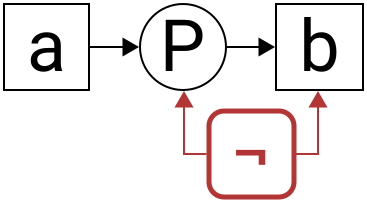
\includegraphics[height=3em]{gfx/theory/negationNode1.pdf}}}
			\quad\Leftrightarrow\quad
			&\exists\ a\ {\color{rot}\lnot\exists}\ b: P(a, b) \numberthis \\
			\quad\Leftrightarrow\quad
			&\exists\ a\ {\color{rot}\forall}\ b: {\color{rot}\lnot} P(a, b)
		\end{align*}
		Die Darstellung von Kontexten mit Knoten und Kanten wird schnell unübersichtlich, daher werden stattdessen Boxen verwendet, die die Kindknoten umschließen.
		\begin{align*}
			\vcenter{\hbox{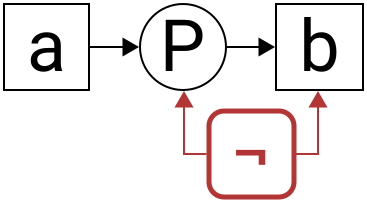
\includegraphics[height=3em]{gfx/theory/negationNode1.pdf}}}
			\quad\Leftrightarrow\quad
			\vcenter{\hbox{\includegraphics[height=3em]{gfx/theory/negationNode2.pdf}}}
		\end{align*}
		Kontexte können nicht nur Konzeptknoten und Relationsknoten enthalten, sondern auch andere Kontexte.
		Hierbei ist zu beachten, dass alle Knoten und Kontexte höchstens einen Elternkontext haben können;
		die Linien zweier Kontextboxen dürfen sich also nicht schneiden.
		\begin{align*}
			\vcenter{\hbox{
\includegraphics[height=3em]{gfx/theory/negationNode3.pdf}}}
			\quad\Leftrightarrow\quad
			&{\color{rot}\lnot\exists}\ a\ {\color{rot}\lnot\exists}\ b: P(a, b) \numberthis \\
			\quad\Leftrightarrow\quad
			&{\color{rot}\forall}\ a\ \exists\ b: P(a, b)
		\end{align*}
		\begin{align*}
			\vcenter{\hbox{
\includegraphics[height=3.75em]{gfx/theory/negationNode4.pdf}}}
			\quad\Leftrightarrow\quad
			&\exists\ a, b: {\color{rot}\lnot}({\color{rot}\lnot} P(a, b) \land {\color{rot}\lnot} R(b, a)) \numberthis \\
			\quad\Leftrightarrow\quad
			&\exists\ a, b: P(a, b)\ {\color{rot}\lor}\ R(b, a)
		\end{align*}
	\item \textbf{Koreferenzkanten (\textit{coreference links}):}
		Entspricht der Äquivalenzrelation.
		\begin{align}
			\vcenter{\hbox{\includegraphics[height=3.75em]{gfx/theory/coreferenceEdge.pdf}}}
			\quad\Leftrightarrow\quad
			&\exists\ a, b: P(a, b) \land \lnot\exists\ x: {\color{rot}a = x \land x = b} \\
			\quad\Leftrightarrow\quad
			&\exists\ a, b: P(a, b) \land {\color{rot}a \neq b} \nonumber
		\end{align}
\end{itemize}

\subsection{Dominierende Knoten}%
\label{sec:theory:cg:domnodes}

Nicht alle Graphen, die sich mit den soeben beschriebenen Syntaxelementen bilden lassen, sind gültige Konzeptgraphen.
Die Einschränkung, dass alle Knoten und Kontexte höchstens einen Elternkontext haben dürfen, wurde bereits erwähnt.
Eine weitere Einschränkung ist das Verbot nicht dominierender Knoten (\textit{dominating nodes}).
Was genau dies bedeutet, wird im Folgenden erläutert. Zuerst müssen Konzeptgraphen jedoch formal spezifiziert werden.
\begin{align*}
	G :=\ &(V, E) \\
	V \ni\ &\top, E \supseteq \{ (\top, v): v \in V \land \lnot\exists\ c \in V: context(c) \land (c, v) \in E \} \\
	concept(v) :\Leftrightarrow\ &\text{$v \in V$ ist ein Konzeptknoten} \\
	relation(v) :\Leftrightarrow\ &\text{$v \in V$ ist ein Relationsknoten} \\
	context(v) :\Leftrightarrow\ &\text{$v \in V$ ist ein Kontext, es gilt $context(\top)$} \\
	neg(v) :\Leftrightarrow\ &\text{$v \in V$ ist ein Negationskontext} \\
	a \leq b :\Leftrightarrow\ & (\exists\ x \in V: a \leq x \land x \leq b) \numberthis \\
	& \lor (context(b) \land (b, a) \in E) \\
	& \lor (\exists\ c \in V: context(c) \land (c, a) \in E \land (c, b) \in E)
\end{align*}
Um die nachfolgenden Definitionen einfacher zu machen, wird der globale Kontext $\top$ eingeführt.
$\top$ enthält alle Knoten, die keinen Elternkontext haben.
$\leq$ ist eine Quasiordnung und bildet die \textit{enthalten-in}-Relation zwischen Knoten ab, d.~h.\ $a \leq b$ gdw.\ $a$ nicht außerhalb der Box des Elternkontextes von $b$ liegt.
Das größte Element gemäß $\leq$ ist also immer $\top$.

Jeder gültige Konzeptgraph muss dominierende Knoten haben.
\begin{align*}
	\vcenter{\hbox{\includegraphics[height=3.75em]{gfx/theory/dominatingNodeViolation1.pdf}}}
	\quad
	\text{\color{rot}$\lightning$ Keine dominierenden Knoten, da $b \leq P$.}
\end{align*}

\section{Stanford CoreNLP}%
\label{sec:theory:nlp}

\section{Modellierung von Hinge-Loss-MRFs mit PSL}%
\label{sec:theory:psl}

% !TEX root = ../main.tex
%
\chapter{Vorgeschlagenes Wissensgraph\-konstruktions\-verfahren}%
\label{sec:text2kg}

Auf Basis der vorgestellten Konzeptgraphen, CoreNLP und PSL wird im folgenden Kapitel ein Verfahren für die online Konstruktion eines Wissensgraphen aus natürlichsprachlichen Textnachrichten aufgebaut.
Der Fokus liegt dabei primär auf der generellen Architektur des Verfahrens.
Das Resultat ist also als Proof-of-Concept zu verstehen, auf dessen Basis praxistaugliche Systeme konzipiert werden können.

\begin{figure}[h]
	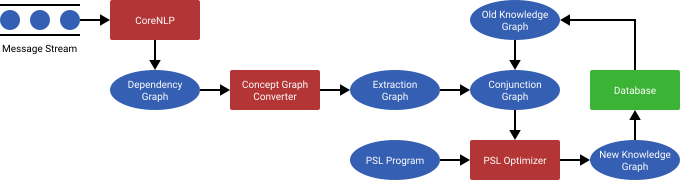
\includegraphics[width=\textwidth]{gfx/text2kg/architecture.pdf}
	\caption{Grobes Architekturdiagramm der Konstruktionspipeline}\label{fig:text2kg:architecture}
\end{figure}
Das im Folgenden vorgestellte Verfahren folgt einem dreistufigen Pipeline-Modell:
\begin{enumerate}
	\item Mittels CoreNLP wird eine eintreffende Textnachricht in einen Abhängigkeitsgraphen transformiert.
	\item Der resultierende Abhängigkeitsgraph wird in einen sog.\ Extraktionsgraphen umgewandelt.
		Hierbei handelt es sich um einen Konzeptgraphen, der den Inhalt der Nachricht formal repräsentiert.
	\item Der Extraktionsgraph wird mit dem bestehenden Wissensgraphen verschmolzen.
		Dies entspricht der Konjuktion der durch die beiden Graphen repräsentierten logischen Ausdrücke.
		Der resultierende Konjunktionsgraph wird als Eingabe für ein PSL-Programm verwendet, welches auf Basis des hinzugekommenen Wissens neue Beziehungen im Wissensgraphen inferiert.
\end{enumerate}
Die Beschreibung dieser Pipeline erfolgt in vier Abschnitten.
In \treft{sec:text2kg:implementation} wird kurz die technische Umsetzung erläutert.
\treft{sec:text2kg:ontology} beschreibt anschließend die Ontologie der konstruierten Wissensgraphen.
Nach diesen strukturellen Betrachtungen wird schließlich in \treft{sec:text2kg:nlp} und \treft{sec:text2kg:psl} die Transformation von Text zu Extraktionsgraph, bzw.\ von Extraktionsgraph zu Wissensgraph beschrieben.

\section{Implementation}%
\label{sec:text2kg:implementation}

Das in den folgenden Abschnitten beschriebene Verfahren wurde im Rahmen dieser Arbeit prototypisch implementiert.
Bei der Wahl der hierfür verwandten Technologien wurde darauf Wert gelegt, dass eine möglichst nahtlose Integration der Komponenten möglich ist.
Sowohl CoreNLP~\cite{CoreNLP} als auch die PSL-Referenzimplementation~\cite{PSL} sind JVM-Bibliotheken.
Diese Arbeit wurde daher ebenfalls in einer JVM-Sprache implementiert.

Hierfür wurde Clojure gewählt, ein moderner Lisp-1-Dialekt, mit einem Fokus auf funktionale Programmierung, unveränderliche Datenstrukturen und gleichzeitiger Interoperabilität mit objektorientierten Bibliotheken.
Andere JVM-Sprachen, wie z.~B. Java, Scala oder Groovy, wurden ausgeschlossen, da sie sich während des Entwicklungsprozesses als hinderlich erwiesen haben.
Der Hauptgrund hierfür ist, dass CoreNLP bei der Initialisierung diverse Modelle laden muss.
Bei Verwendung eines modernen Desktop-Rechners benötigt dies ca.~20 Sekunden, auf langsamerer Hardware teils mehrere Minuten;
diese Wartezeiten waren ein stark verlangsamender Faktor beim entwickeln.
Da Clojure ein Lisp ist, unterstützt es traditionsgemäß \textit{REPL Driven Development}.
Statt nach jeder Änderung die Anwendung neu zu starten und die Modelle erneut zu laden, kann so lediglich der geänderte Bytecode in den laufenden Prozess injiziert werden;
die geladenen Modelle bleiben dabei im Speicher und die Änderung kann ohne weitere Wartezeit getestet werden.
Durch die Wahl von Clojure konnte die Entwicklung deutlich beschleunigt werden.

\section{Wissensgraphontologie}%
\label{sec:text2kg:ontology}

Bevor Wissensgraphen konstruiert werden können, muss spezifiziert sein, wie genau diese aussehen sollen.
Um komplexe logische Beziehungen ausdrücken zu können, wird die bereits vorgestellte Konzeptgraph-Struktur verwendet.
Dabei bleibt allerdings offen, welche Prädikate vorkommen können und welche Bedeutung sie haben.
Außerdem ist unklar, wie mit Konzeptgraphen modale Aussagen ausgedrückt werden.
Damit aus einem Konzeptgraphen ein Wissensgraph wird, muss eine Ontologie gegeben sein, welche diese offenen Punkte schließt.
Im Folgenden wird beschrieben, wie genau die in dieser Arbeit verwendete Ontologie aufgebaut ist.

\subsection{Verwendete Prädikate}%
\label{sec:text2kg:ontology:pred}

\subsection{Modale Kontexte}%
\label{sec:text2kg:ontology:modal}

Im zweiten Schritt wird nun geklärt, wie Modalität repräsentiert wird.
Beispiele für modale Aussagen sind:
\begin{center}
	\textit{``I {\color{blau}think} that {\color{rot}the book is good}.''}\\
	\textit{``{\color{rot}I} {\color{blau}don't want} to {\color{rot}go to the beach}.''}
\end{center}
Die beiden Teilaussagen \textit{\color{rot}``the book is good''} und \textit{\color{rot}``I go to the beach''} sind offensichtlich nicht unbedingt wahr, sondern beschreiben Möglichkeiten, die in Abhängigkeit von \textit{\color{blau}think} bzw.\ \textit{\color{blau}don't want} wahr oder falsch werden könnten.
Ob die Aussagen wahr werden, hängt davon ab, inwiefern das Denken oder Wollen einer Person mit der Realität übereinstimmt.
Dies ist je nach Person stark verschieden; manche tendieren dazu die allgemein als wahr akzeptierten Aussagen zu denken bzw.\ entsprechend ihrer Wünsche zu handeln, andere nicht.

Um derartige Möglichkeiten und Notwendigkeiten direkt zu repräsentieren, reichen die vorgestellten Konzeptgraphen mit Negationskontexten nicht aus.
Sowa hat dieses Problem ebenfalls erkannt und daher weitere Kontexttypen eingeführt.
Die Beschreibung dieser zusätzlichen Kontexttypen ist allerdings oftmals zu unpräzise für eine eindeutige Übersetzung in die Prädikatenlogik.
Aufbauend auf Sowas Ideen wird in dieser Arbeit daher eine abgeschwächte Variante modaler Kontexte eingeführt, die die Übersetzbarkeit in die Prädikatenlogik erster Ordnung bewahrt.
Da die zuvor vorgestellten Konzeptgraphen bereits vollständig und korrekt sind, handelt es sich bei diesen modalen Kontexten also lediglich um eine Kurzschreibweise.

Insgesamt gibt es durch die Erweiterung um modale Kontexe nun folgende vier Kontexttypen:
\begin{multicols}{2}
	\flushleft\begin{enumerate}
		\item Positiver Aktualkontext
		\item Negativer Aktualkontext
		\item Positiver Möglichkeitskontext
		\item Negativer Möglichkeitskontext
	\end{enumerate}
\end{multicols}
Die modale Notwendigkeit hat keine eigenen Kontexttypen erhalten, um konsistent zur Quantisierung in Konzeptgraphen zu bleiben.
So, wie der Allquantor in Konzeptgraphen durch Negation der negierten existenzquantisierten Aussage ausgedrückt wird, wird die Notwendigkeit durch Negation der negativen Möglichkeit ausgedrückt.

Da es nun vier Kontexttypen gibt, muss die Konzeptgraphsyntax leicht angepasst werden, um zwischen den verschiedenen Typen differenzieren zu können:
\begin{figure}[h]
	\centering
	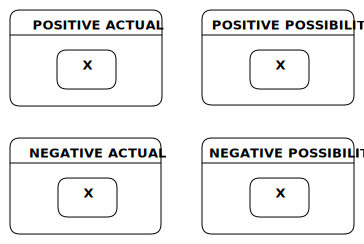
\includegraphics[scale=0.6]{gfx/text2kg/contextTypes.pdf}
	\caption{Konzeptgraphsyntax für modale Kontexte}\label{fig:text2kg:contextTypes}
\end{figure}

\paragraph{Positiver Aktualkontext}
Dieser Kontexttyp hat keinen Einfluss auf die Bedeutung der enthaltenen Knoten.
Er entspricht in etwa der Klammerung in der Prädikatenlogik.
Das \textit{Sheet of Assertion}~$\top$ ist ein solcher Kontext, abgesehen davon tauchen positive Aktualkontexte allerdings nicht auf;
sie werden hier lediglich der Vollständigkeit halber erwähnt.
\begin{align}
	\vcenter{\hbox{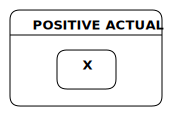
\includegraphics[scale=0.6]{gfx/text2kg/positiveActual.pdf}}}
	\Leftrightarrow
	\vcenter{\hbox{\includegraphics[scale=0.6]{gfx/text2kg/x.pdf}}}
	\Leftrightarrow
	\exists x: label(x, \text{``X''})
\end{align}

\paragraph{Negativer Aktualkontext}
Entspricht dem bisherigen Negationskontext.
\begin{align}
	\vcenter{\hbox{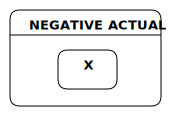
\includegraphics[scale=0.6]{gfx/text2kg/negativeActual.pdf}}}
	\Leftrightarrow
	\lnot \exists x: label(x, \text{``X''})
\end{align}

\paragraph{Positiver Möglichkeitskontext}
Dieser Kontexttyp bildet die modale Möglichkeit ab.
Um die Mächtigkeit der Prädikatenlogik beizubehalten, wird hierfür keine fundamental neue Struktur eingeführt.
Es wird stattdessen die Tatsache ausgenutzt, dass sich die modalen Operatoren gemäß der Mögliche-Welten-Interpretation analog zu den prädikatenlogischen Quantoren verhalten.
\begin{align*}
	{\color{rot}\square} P(x)\ &\Leftrightarrow \lnot {\color{blau}\lozenge} \lnot P(x) \\
	{\color{rot}\forall} w: world(w) \rightarrow P_w(x)\ &\Leftrightarrow \lnot {\color{blau}\exists} w: world(w) \land \lnot P_w(x) \numberthis
\end{align*}
Die Aussage \textit{``$P(x)$ gilt notwendigerweise''}, wird also als \textit{``Es gibt keine Welt $w$ in der $P_w(x)$ nicht gilt''} aufgefasst.
Statt von Welten, wird in modalen Konzeptgraphen allerdings von Kontexten gesprochen.

\paragraph{Negativer Möglichkeitskontext}
Lediglich eine Kurzschreibweise für einen positiven Möglichkeitskontext der einen negativen Aktualkontext umgibt.

\section{NLP-Phase}%
\label{sec:text2kg:nlp}

\section{Graphkonstruktionsphase}%
\label{sec:text2kg:psl}

% !TEX root = ../main.tex
%
\chapter{Auswertung}
\label{sec:evaluation}

\section{Testmethode}
\label{sec:evaluation:methodology}

\section{Ergebnisse}
\label{sec:evaluation:results}

% !TEX root = ../main.tex
% chktex-file 46
\chapter{Zusammenfassung}%
\label{sec:conclusion}

Abschließend wird nun zusammengefasst, inwiefern das in~\ref{sec:intro:goals} beschriebene Ziel einer erweiterbaren, parallelisierbaren Wissensgraph-Konstruktion aus Kommunikationsdaten erreicht wurde.
Hierfür werden in~\ref{sec:conclusion:review} die erreichten Teilziele betrachtet.
Anschließend wird in~\ref{sec:conclusion:todo} ein Ausblick auf Möglichkeiten der Weiterentwicklung des Systems gegeben.

\section{Rückblick}%
\label{sec:conclusion:review}

\begin{figure}[h]
	\centering
	
\includegraphics[width=0.65\textwidth]{gfx/conclusion/overview.pdf}
	\caption{Grober Aufbau des Konstruktionsverfahrens}\label{fig:conclusion:overview}
\end{figure}
In Kapitel~\ref{sec:text2kg} wurden Lösungen für die drei wesentlichen Teilprobleme Ontologie, Sprachverarbeitung und Grapherweiterung beschrieben.
Die drei Teillösungen bilden zusammen ein Konstruktionsverfahren, welches dem zu Anfang beschriebenen Aufbau entspricht.

\paragraph{Ontologie}
Die Wissensgraphontologie basiert auf Konzeptgraphen.
Im Gegensatz zu den Fakten-Tripel basierten semantischen Netzen, die lediglich beschreiben, welche Beziehungen zwischen Konzepten existieren, kann mittels Konzeptgraphen auch beschrieben werden, welche Beziehungen nicht, oder nur möglicherweise existieren.
Die konstruierten Wissensgraphen haben also eine deutlich höhere Ausdrucksstärke, als z.~B. NELL oder der Google~Knowledge~Graph.
Diese Ausdrucksstärke ist notwendig, um die Komplexität natürlichsprachlicher Aussagen sinnvoll abbilden zu können.

Damit die Konzeptgraphen eine möglichst präzise Semantik haben, muss die Semantik der verwendeten Relationen beschrieben werden.
Es wurde daher ein möglichst minimales Set von Relationen definiert~\tref{sec:text2kg:ontology:pred}, welches zur Beschreibung einer Vielzahl natürlichsprachlicher Aussagen geeignet ist.

Eine der in~\ref{sec:intro:goals} beschriebenen Anforderungen an das Konstruktionsverfahren ist die Erweiterbarkeit, d.~h.\ die prinzipielle Möglichkeit nicht natürlichsprachliche Eingaben einzufügen.
Konkret bedeutet dies, dass z.~B. ein Bild in denselben Wissensgraph eingefügt werden kann, in den auch Textnachrichten eingefügt werden.
Da die gewählten Konzeptgraph-Relationen nicht speziell für natürliche Sprache ausgelegt sind, ist dies prinzipiell möglich;
es gibt keine Relationen, die bestimmte grammatikalische Konstrukte oder Wortarten abbilden.
Wie die Integration anderer Eingabearten im Detail aussehen könnte, war jedoch nicht Teil der Aufgabenstellung und wurde daher nicht näher untersucht.

\paragraph{Sprachverarbeitung}
Für die Transformation einer Nachricht in einen Konzeptgraphen wird das Stanford~CoreNLP Framework mit einer Menge von Transformationsregeln~\tref{sec:text2kg:nlp:transform} kombiniert, welche die von CoreNLP gefundenen Strukturen auf äquivalente Konzeptgraph-Strukturen abbilden.

\paragraph{Grapherweiterung}
Das Einfügen des aus einer Nachricht extrahierten Konzeptgraphen in einen bestehenden Wissensgraphen erfolgt mittels PSL.\@
Im Rahmen dieser Arbeit wurde PSL erstmals im Kontext einer Konzeptgraph-basierten Wissensgraph-Konstruktion eingesetzt.
Es wurde ein Set von PSL-Regeln~\tref{sec:text2kg:psl:inference} vorgestellt, welches den Einsatz in diesem Kontext exemplarisch aufzeigt.

Neben der Erweiterbarkeit war auch die Parallelisierbarkeit eines der in~\ref{sec:intro:goals} beschriebenen Ziele.
Durch die Wahl von PSL für die Grapherweiterung wurde diese Anforderung prinzipiell erfüllt.
Das für die Inferenz verwendete ADMM-Verfahren lässt sich gut verteilt lösen.
In~\cite[Kapitel 10]{Boyd2011} wird beschrieben, wie sich ADMM mit verteilten Programmiermodellen, wie z.~B. Map-Reduce oder Pregel, implementieren lässt.
Aufbauend darauf, wird in~\cite{Lubell-Doughtie2013} eine konkrete Map-Reduce-basierte Implementation vorgestellt.
PSL ist prinzipiell also für den Einsatz in Cluster-Umgebungen geeignet.
In der im Rahmen dieser Arbeit erstellten Implementation wurde jedoch die Single-Machine ADMM-Implementation der PSL-Referenzimplementation verwendet, da diese für einen Prototypen völlig ausreichend ist.

Das Ziel ein erweiterbares, parallelisierbares Wissensgraph-Konstruktionsverfahren für Kommunikationsdaten zu konzipieren wurde somit prinzipiell erreicht.
Nichts desto trotz gibt es noch zahlreiche Möglichkeiten das vorgestellte Verfahren weiterzuentwickeln.

\section{Ausblick}%
\label{sec:conclusion:todo}

Im Folgenden wird ein Überblick über Möglichkeiten der Weiterentwickung und offen gebliebene Fragestellungen gegeben.

\paragraph{Verbessern der Testmethode}
Ein Problem bei der Konzeption des Verfahrens war der Umstand, dass es keine Testdaten mit Referenzergebnissen gibt, anhand derer Änderungen am Verfahren bewertet werden können.
Die Qualität vieler Entscheidungen, wie z.~B. der Wahl der Regelgewichte, konnte daher nur auf Basis manuell durchgeführter, stichprobenartiger Tests bewertet werden.

Das Entwickeln eines Testdaten-Sets, mit dem sich die Performance eines Wissensgraph-Konstruktionsverfahrens repräsentativ empirisch messen lässt, ist wichtig, um ein systematisches Weiterentwickeln des Verfahrens zu ermöglichen.
Das in dieser Arbeit verwendete Enron E-Mail Datenset ist potentiell ein guter Ausgangspunkt hierfür.
Zu klären ist, welche Art von Informationen die Referenzergebnisse enthalten und wie eine umfangreiche Menge solcher Referenzergebnisse konstruiert werden kann.

\paragraph{NLP-Phase}
Im vorgestellten Verfahren wird lediglich ein Teil der von CoreNLP extrahierten Informationen in Konzeptgraph-Strukturen übersetzt.
Durch die Integration bislang ungenutzter Abhängigkeitstypen ließe sich die Qualität der Ergebnisse, wie in~\ref{sec:evaluation:quality:results}~Anfrage~2 gezeigt, deutlich verbessern.

Außerdem sollte die verwendete Heuristik zur Übersetzung von natürlichsprachlicher Negation in negative Kontexte verbessert werden.
In~\ref{sec:evaluation:quality:results}~Anfrage~4 wird dies deutlich.
Ein Ansatz hierfür ist z.~B. das Nutzen des CoreNLP Natural Logic Annotators~\cite{MacCartney2007}, welcher u.~a.\ Quantoren, Negationen und die zugehörigen Scopes, d.~h.\ die modifizierten Token, erkennt.

\paragraph{PSL-Phase}
Die verwendeten domänenspezifischen Regeln und das domänenspezifische Vorwissen sind bislang sehr rudimentär.
In künftigen Arbeiten könnten vorhandene Wissensbasen, wie z.~B. NELL~\cite{Carlson2010} oder YAGO~\cite{YAGO}, in die PSL-Inferenz integriert werden.

Neben der Nutzung domänenspezifischen Wissens, besteht außerdem Verbesserungspotential bei der Nutzung von Kontexten in der Inferenz.
Bislang werden Kontexte nur benutzt, um die Richtung von $inst$-Relationen zu ermitteln.
Das Inferieren des $actual$-Attributs von Möglichkeitskontexten~\tref{sec:text2kg:ontology:modal} zur Bestimmung der Glaubwürdigkeit von Aussagen wäre z.~B. eine sinnvolle Erweiterung des Verfahrens.

\paragraph{Inferenz}
Wie~\treft{sec:evaluation:time} gezeigt hat, besteht noch Verbesserungsbedarf bei der Geschwindigkeit der PSL-Inferenz, bevor das Verfahren in der Praxis einsetzbar ist.
Um dies zu erreichen, ist die Kombination verschiedener Ansätze denkbar:
\begin{enumerate}
	\item Nutzen einer Cluster-fähigen ADMM-Implementation, statt der PSL-Referenz\-implementation.
		Hierfür könnte z.~B. die zuvor erwähnte Hadoop Map-Reduce Implementation~\cite{Lubell-Doughtie2013} verwendet werden.
	\item Weiterentwicklung von BOCI, sodass wachsende Eingabemengen unterstützt werden.
		Bereits im ursprünglichen Paper~\cite[Abschnitt 6]{Pujara2015} wird dies als offene Fragestellung für folgende Arbeiten genannt.
		Mittels des Inferenz-Budgets könnte dann die Inferenzdauer nahezu beliebig verringert werden, sofern dafür eine entsprechende Verschlechterung der Inferenzqualität hingenommen wird.
\end{enumerate}


% --------------------------
% Back matter
% --------------------------
\appendix\cleardoublepage\
% !TEX root = ../main.tex
% chktex-file 46

\chapter{Anhang}%
\label{sec:appendix}

\section{Verwendete Testnachrichten}%
\label{sec:appendix:msgs}

Die Testnachrichten 1--7 stammen aus dem Thread \texttt{bin1/363227} des Enron Threads Corpus~\cite{EnronThreads}.
Die Testnachricht 8 wurde nachträglich hinzugefügt, da in den vorherigen Nachrichten keine Negation vorkam.
Da das implementierte Wissensgraph-Konstruktionsverfahren nicht speziell für E-Mails ausgelegt ist, wird nicht zwischen Absender und Absender-Adresse unterschieden.
Die Absender- und Empfänger-Adressen in den Rohdaten wurden daher durch die Namen der Absender bzw. Empfänger ersetzt.
Abgesehen von dieser Änderung wurden die Inhalte und Absendezeitpunkte der Mails unverändert übernommen.
\inputminted{clojure}{data/evaluation/testdata.clj}

\section{Verwendete Testanfragen}%
\label{sec:appendix:queries}

Zur Evaluation des aus den Testnachrichten konstruierten Wissensgraphen wurden drei Testanfragen verwendet, die jeweils verschiedene Aspekte des Graphen betrachten.
Die Anfragen sind in der Sprache Cypher des Neo4j-Graphdatenbanksystems~\cite{Neo4j} geschrieben.
Die Tests wurden mit Neo4j~3.2.6 und dem Graph Algorithms Plugin~3.2.2.1~\cite{GraphAlgo} durchgeführt.

\subsection{Personen}%
\label{sec:appendix:queries:people}

\inputminted{cypher}{data/evaluation/people.cql}
Diese Anfrage arbeitet im Wesentlichen in zwei Schritten.
Im ersten Schritt wird der Teilgraph aller Konzepte gebildet, die Instanz von \textit{person} und nicht Instanz von \textit{I} oder \textit{you} sind.
Im zweiten Schritt wird dann die Menge aller über $inst$-Kanten schwach zusammenhängender Komponenten des Teilgraphen ermittelt.
Die $label$ der Konzepte innerhalb einer Zusammenhangskomponente sind die Namen bzw.\ Bezeichner, die dieselbe Person in verschiedenen Nachrichten hat.

Der Grund für diesen Aufbau ist, dass eine Person als ein Konzept mit gewissen charakterisierenden Eigenschaften verstanden werden kann.
Die Existenz von $inst(A, B)$ zwischen zwei Personen-Konzepten $A, B$ bedeutet, dass $B$ die charakterisierenden Eigenschaften von $A$ besitzt und somit beide Konzepte auf die selbe Person verweisen.
Für die Modellierung dieser Idee werden keine Koreferenzkanten verwendet, da zwei Konzepte, die auf dieselbe Person verweisen, dennoch verschieden sein können; $B$ könnte z.~B. ein Konzept sein, welches die Person $A$ zu einem bestimmten Zeitpunkt repräsentiert.

\subsection{Ereignisse und Termine}%
\label{sec:appendix:queries:events}

\inputminted{cypher}{data/evaluation/personTimeAction.cql}
Diese Anfrage ermittelt die Liste der $label$ aller $relation$-Konzepte und ihrem Patiens, deren Agens die Person ist, die durch \textit{Duane Seppi} bezeichnet wird.
Sofern bekannt, wird den Relationskonzepten der Zeitpunkt zugeordnet, deren Patiens sie sind.

\subsection{Personenbezogene Daten}%
\label{sec:appendix:queries:numbers}

\inputminted{cypher}{data/evaluation/numbers.cql}
Diese Anfrage ermittelt zuerst alle Konzepte, die Instanz von \textit{number} sind und zugleich Patiens einer Person sind;
die Patiens-Relation zwischen einer Person und einem anderen Konzept wird benutzt, um eine Zugehörigkeit auszudrücken.
Das Ergebnis ist also die Menge aller Nummern und den Personen, denen sie gehören.
Um zu bestimmen, um was für eine Art von Nummer es sich dabei jeweils handelt, wird anschließend für jede Numme $B$ die Menge aller Konzepte $A$ bestimmt, für die $inst(A, B)$ gilt.

\subsection{Positive und negative Aussagen}%
\label{sec:appendix:queries:neg}

\inputminted{cypher}{data/evaluation/personNegationAction.cql}
Diese Anfrage ermittelt zuerst alle Relationen, die von einem Kontext umgeben sind, der den Inhalt einer Nachricht beschreibt, die von \textit{John Doe} gesendet wurde.
Anschließend wird für jede Relation geprüft, ob sie negative umgebende Kontexte hat.
Da bereits in der NLP-Phase doppelte Verneinungen vereinfacht werden, müssen diese nicht beachtet werden.
Es ist daher zwischen drei Fällen zu unterscheiden:
\begin{enumerate}
	\item \textbf{\texttt{POSITIVE}:}
		Die Relation hat keine negativen umgebenden Kontexte und ist somit selbst positiv.
	\item \textbf{\texttt{NEGATIVE}:}
		Die Relation hat einen negativen umgebenden Kontext, deren einziges Kind sie ist.
		In diesem Fall ist die Relation negiert.
	\item \textbf{\texttt{CONDITIONAL}:}
		Die Relation hat mehrere negative umgebende Kontexte oder ist nicht einziges Kind ihres negativen umgebenden Kontextes.
		In diesem Fall ist die Existenz der Relation abhängig von der Existenz anderer Konzepte.
		Prinzipiell ließen sich diese Abhängigkeiten abfragen, der Einfachheit halber, wird dies hier jedoch nicht getan.
\end{enumerate}
Diese Anfrage ist ein gutes Beispiel dafür, dass mit einer Graph-Anfragesprache, in diesem Fall Cypher, Kontexte nur recht umständlich berücksichtigt werden können.
Das Entwickeln eines speziell für Konzeptgraphen ausgelegten Anfragesystems ist daher empfehlenswert, um die Syntax komplexerer Anfragen verständlich zu halten.

\section{Laufzeitergebnisse}%
\label{sec:appendix:perf}

Es folgt eine Tabelle mit den gemessenen Laufzeitergebnissen.
Für jede Nachricht $m_i$ werden die folgenden Daten angegeben:
\begin{enumerate}[noitemsep]
	\item Die Einfügedauer $t_i$ in Sekunden.
	\item Die Veränderung der Einfügedauer $\Delta t_i = t_i - t_{i - 1}$.
	\item Die Anzahl $|\mathbb{C}_i|$ geschlossener Grundatome beim Einfügen von $m_i$.
	\item Die Anzahl neuer Konzepte $c_i$ in $m_i$, d.~h.\ Konzepte mit einem $label$, welches in den vorigen Nachrichten noch nicht vorgekommen ist.
	\item Der Korrelationskoeffizient $Kor_i(t, \mathbb{C}) = Kor({(t_j)}_{j = i, \dots, 57}, {(|\mathbb{C}_j|)}_{j = i, \dots, 57})$.
	\item Der Korrelationskoeffizient $Kor_i(\Delta t, c) = Kor({(\Delta t_j)}_{j = i, \dots, 57}, {(c_j)}_{j = i, \dots, 57})$.
\end{enumerate}

Die Nachrichten $m_1, \dots, m_{24}$ stammen aus \texttt{bin1/300249}, $m_{25}, \dots, m_{32}$ sind die für die Qualitätsuntersuchung verwendeten Nachrichten aus \texttt{bin1/363227}~\tref{sec:appendix:msgs}, $m_{33}, \dots, m_{57}$ stammen aus \texttt{bin5/350143}.
\csvreader[
	longtable={rrrrrS[group-digits=false]S[group-digits=false]},
	separator=comma,
	table head={\toprule$i$ & $t_i$ & $\Delta t_i$ & $|\mathbb{C}_i|$ & $c_i$ & {$Kor_{i}(t, \mathbb{C})$} & {$Kor_{i}(\Delta t, c)$}\\\midrule\endhead\bottomrule\endfoot}, % chktex 21
	late after line=\\,
	head to column names
]{data/evaluation/perfBig.csv}{}{\i& $\time$& $\dtime$& $\input$& $\concepts$& \icorrel& \ccorrel}

%
{%
\setstretch{1.1}
\renewcommand{\bibfont}{\normalfont\small}
\setlength{\biblabelsep}{0pt}
\setlength{\bibitemsep}{0.5\baselineskip plus 0.5\baselineskip} % chktex 1
\setcounter{biburllcpenalty}{9000}
\setcounter{biburlucpenalty}{9999}
\printbibliography[nottype=online]
\printbibliography[heading=subbibliography,title={Webseiten},type=online]
}
\cleardoublepage\

\listoffigures
\cleardoublepage\

\pdfbookmark[0]{Erklärung}{Erklärung}
\chapter*{Erklärung zur Bachelorarbeit}%
\label{sec:declaration}
\thispagestyle{empty}

Ich, \thesisName\ (Matrikel-Nr. \thesisMatNr), versichere, dass ich die Bachelorarbeit mit dem Thema \textit{\thesisTitle} selbstständig verfasst und keine anderen als die angegebenen Quellen und Hilfsmittel benutzt habe.
Die Stellen der Arbeit, die ich anderen Werken dem Wortlaut oder dem Sinn nach entnommen habe, wurden in jedem Fall unter Angabe der Quellen der Entlehnung kenntlich gemacht.
Das Gleiche gilt auch für Tabellen, Skizzen, Zeichnungen, bildliche Darstellungen usw.
Die Bachelorarbeit habe ich nicht, auch nicht auszugsweise, für eine andere abgeschlossene Prüfung angefertigt.
Auf §~63~Abs.~5 HZG wird hingewiesen.

\bigskip

\noindent\textit{\thesisUniversityCity, \thesisDate}

\smallskip

\begin{flushright}
	\begin{minipage}{7cm}
		\rule{\textwidth}{1pt}
		\centering\thesisName\
	\end{minipage}
\end{flushright}

\clearpage
\newpage

% **************************************************
% End of Document CONTENT
% **************************************************
\end{document}
